\newpage

\section{背景知识与技术}

在探讨 HORAE 的设计之前,有必要了解一些关键的背景知识和技术,这些将为后续的研究提供理论和实践基础。

\subsection{服务监管系统架构}

\begin{figure}[ht]
    \centering
    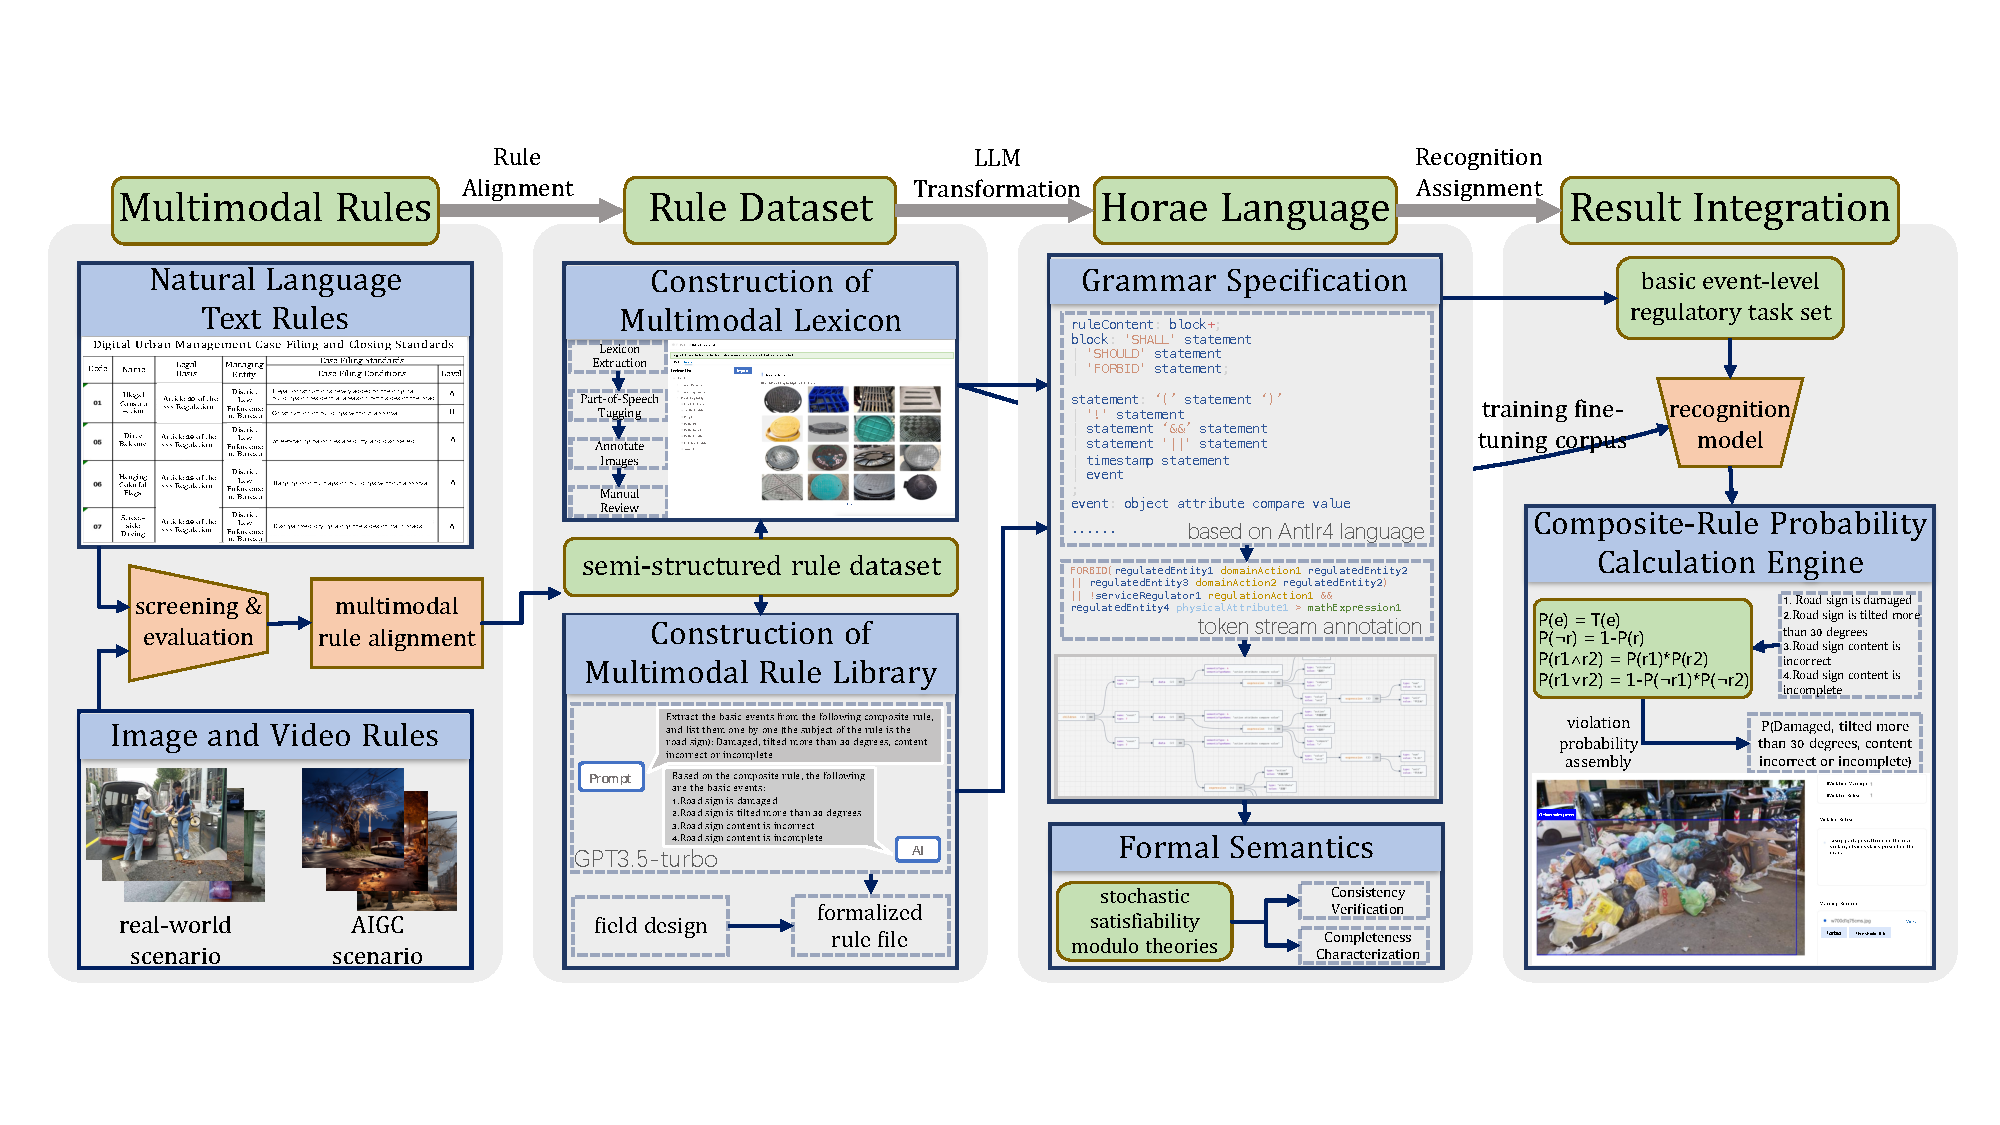
\includegraphics[width=\linewidth]{111.pdf}
    \caption{\label{fig:total-struct}服务监管系统架构}
\end{figure}

 HORAE 是构建高效服务监管系统的核心要素,它在整个监管框架中扮演着至关重要的角色。\autoref{fig:total-struct}描述了服务监管系统的工作流程和架构概览,具体包括:

\begin{itemize}
    \item \textbf{数据集的整合与预处理:} 系统从多模态的规则数据集着手,这些数据集可能包含文本、语音、图像等多种格式的规则信息。
    \item \textbf{规则数据库的初步构建:} 通过应用 HORAE ,原始的多模态规则数据被转换成一种半结构化的格式,进而形成规则数据库。这一步骤是将非结构化数据转换为机器可读格式的关键环节。
    \item \textbf{语法规范与处理:} 遵守既定的语法规范,系统对半结构化的规则数据进行进一步的精细化处理,提炼出规则的深层次结构,并构建成语法树。语法树的构建为后续的语义分析和规则执行提供了清晰的逻辑框架。
    \item \textbf{语义建模与检测:} 在语法树的基础上,系统进行语义建模,将规则中的自然语言转化为机器可理解的语义表达。同时,系统执行语义检测,确保规则的一致性和无歧义性,避免潜在的逻辑矛盾。
    \item \textbf{大模型服务监管的实现:} 最后,经过上述步骤处理的规则被应用于大模型驱动的服务监管工作中。大模型凭借其强大的数据处理和智能识别能力,能够高效地执行监管任务,实现服务的自动化和智能化监管。
\end{itemize}

整个服务监管系统的架构设计旨在实现规则的高效管理、精准执行和智能监管。 HORAE 的设计和应用,确保了规则从原始数据到最终执行的每一步都准确无误,为服务监管的自动化和智能化提供了坚实的基础。通过这种系统化的方法,本研究能够应对日益增长的监管需求,提高监管的效率和效果,确保服务的合规性和安全性。

\subsection{Antlr语法分析器生成工具}

Antlr\cite{parr2004s},全称为“ANother Tool for Language Recognition”,是一款功能强大的语法分析器生成工具,主要用于从语言规范中读取构造语法分析器或者转译器的代码。它有以下几个主要特点:

\begin{itemize}
    \item \textbf{易用性:} Antlr提供了一种简洁、直观的语法表示方式,使得用户能够快速地定义和理解语法规则。
    \item \textbf{强大的解析能力:} Antlr能够处理广泛的语法结构,包括LL(*)\cite{parr2011ll}和LL(k)\cite{parr1995antlr}等。无论是处理简单的文本格式,还是复杂的编程语言,Antlr都能够应对自如。
    \item \textbf{丰富的目标语言支持:} Antlr支持生成多种编程语言的解析器,包括Java、C++、Python、JavaScript等,满足了用户的多样化需求。
    \item \textbf{强大的错误处理机制:} Antlr具有强大的错误处理和恢复机制,使得解析器能够在出错时提供及时的反馈,帮助用户识别和修复问题。
    \item \textbf{易于集成:} Antlr生成的解析器易于集成到用户的应用程序中,无论是作为一个独立的组件,还是作为一个库,都能够轻松实现。
\end{itemize}

Antlr是一款功能强大、易用的语法分析器生成工具,无论是用于编译原理的学习,还是用于实际的语言设计和实现,都是一个理想的选择。

\subsection{大语言模型}
大语言模型\cite{zhao2023survey}(Large Language Models,LLMs)在自然语言处理\cite{zhou2020progress}(Natural Language Processing,NLP)领域中是一个重大的突破。它们代表了深度学习在模拟人类语言理解方面所取得的进展。以下是大语言模型的一些核心特性:

\begin{itemize}
    \item \textbf{规模与复杂性:} 大语言模型利用大量的参数\cite{wei2022emergent}(通常是数十亿到数千亿的数量级)来捕获和理解语言的复杂性。这种规模的模型能够学习到语言的深层结构和细微差别,从而在各种语言任务中展现出优异的性能。
    \item \textbf{预训练与微调:} 这些模型通常首先在大规模的数据集上进行预训练,学习语言的通用表示。预训练阶段使模型能够积累广泛的知识,之后在特定任务上的微调则进一步提升了模型的专业性,优化其性能。
    \item \textbf{上下文理解:} 大语言模型能够理解文本的上下文信息,这使得它们能够生成连贯且富有深度的文本内容。这种上下文感知能力是实现高级语言任务,如理解隐喻、同义等复杂结构的关键。
    \item \textbf{多任务学习:} 它们具有处理多种不同任务的能力,如文本分类、问答、文本生成等。这种多任务学习的能力使得大语言模型可以灵活地应用于广泛的应用场景,表现出强大的适应性和灵活性。
    \item \textbf{生成能力:} 大语言模型不仅能够理解语言,还能够生成语言。这使得它们在创意写作、内容生成和对话系统等领域具有广泛的应用潜力。
\end{itemize}

大语言模型在 HORAE 的设计和实施中发挥了关键作用。它们可以用于增强语言的自动解析能力,提升对语义的理解,并执行复杂的逻辑推理任务。此外,大模型还能够辅助监管者在制定和执行规则时更好地理解和应用语言的细微差别,从而提高服务监管的准确性和效率。

\subsection{随机布尔可满足性}
随机布尔可满足性\cite{chen2021sharp}(Stochastic Boolean Satisfiability, SSAT)是逻辑和计算机科学中的一个概念,它在处理不确定性和概率性问题时非常有用。SSAT是传统布尔可满足性问题\cite{alyahya2022structure}(Boolean Satisfiability Problem, SAT)的扩展,引入了概率因素。以下是SSAT的一些核心概念和应用:

\begin{itemize}
    \item \textbf{概率模型:} 在SSAT中,每个布尔变量被赋予一个满足概率,即该变量为真的可能性。这种概率化表示使得SSAT能够模拟现实世界中的不确定性。
    \item \textbf{逻辑约束:} 与传统的SAT问题类似,SSAT中的公式由布尔逻辑运算符(如AND、OR和NOT)连接的变量组成。不同之处在于,SSAT考虑了每个变量的满足概率。
    \item \textbf{可满足性计算:} SSAT的目标是找到一组变量赋值,使得整个公式的满足概率最大化,或者计算在给定约束下公式满足的概率。
    \item \textbf{应用领域:} SSAT在多个领域都有应用,包括机器学习、人工智能、风险评估和决策支持系统。它特别适用于需要在不确定性下做出决策的场景。
    \item \textbf{算法和求解器:} 解决SSAT问题通常需要专门的算法和求解器。这些工具可以处理复杂的逻辑公式,并计算出满足特定概率阈值的解决方案。
    \item \textbf{与服务监管的联系:} 在 HORAE 的设计中,SSAT可以用来评估监管规则在不同情况下的满足概率,帮助监管者理解规则的潜在影响,并优化规则以提高监管效率。
\end{itemize}

SSAT为 HORAE 提供了一种评估和优化监管规则的新方法。通过考虑概率因素,监管者可以更全面地理解和应对监管环境中的不确定性。

\subsection{Z3-Solver}
Z3-Solver\cite{bjorner2023satisfiability}是一个由Microsoft Research开发的高效SMT(Satisfiability Modulo Theories)求解器,它在形式化验证、程序验证和符号计算等多个领域有着广泛的应用。以下是Z3-Solver的一些关键特性:

\begin{itemize}
    \item \textbf{多种逻辑支持:} Z3-Solver支持多种逻辑,包括但不限于二阶逻辑、量化逻辑和各种片段的一阶逻辑,使其能够解决广泛的数学和逻辑问题。
    \item \textbf{高性能:} Z3-Solver采用了许多先进的优化技术,如按需模型生成、高效的搜索策略和并行处理,以提高求解速度和效率。
    \item \textbf{可扩展性:} 设计上注重可扩展性,Z3-Solver能够处理大规模的问题实例,同时保持相对合理的性能。
    \item \textbf{集成与API:} 提供了丰富的API,支持多种编程语言,包括C++、Python、Scala等,方便开发者将其集成到不同的应用中。
    \item \textbf{应用场景:} Z3-Solver被用于软件和硬件验证、网络安全、优化问题、机器学习模型的验证以及形式化方法教育等领域。
    \item \textbf{定理证明:} 在定理证明中,Z3-Solver可以自动化地证明给定的公式或者查找使其为假的反例,大大简化了证明过程。
\end{itemize}

Z3求解器在 HORAE 的实现中扮演了重要角色,特别是在需要形式化验证和逻辑推理的场景中。通过使用Z3,开发者可以确保监管规则的逻辑正确性,并自动化地验证规则之间的一致性和完整性。

\subsection{SBERT}
SBERT\cite{wang2020sbert}(Sentence-BERT)由德国柏林工业大学的团队开发,基于预训练的语言模型,用于生成句子或段落的嵌入表示。这些嵌入可以用于各种下游任务,如语义相似性评估、文本分类等。以下是SBERT的一些关键特性:

\begin{itemize}
    \item \textbf{预训练模型:} SBERT利用了预训练的Transformer\cite{han2021transformer}模型,这些模型已经在大量文本数据上进行了训练,能够捕捉到语言的深层语义信息。
    \item \textbf{可定制性:} 用户可以根据自己的需求选择不同的预训练模型,甚至可以微调模型参数以适应特定的应用场景。
    \item \textbf{生成嵌入表示:} 这些模型能够将句子或段落转换成固定长度的嵌入向量,这些向量可以用于后续的机器学习任务,如聚类、分类或最近邻搜索。
    \item \textbf{语义相似性评估:} SBERT在语义相似性评估任务中表现出色,它们能够量化句子之间的语义相似度或相关性。
    \item \textbf{跨语言能力:} 一些SBERT模型支持跨语言的文本比较,即使在不同语言之间也能评估文本的相似性。
    \item \textbf{应用场景:} 这些模型被广泛应用于问答系统、对话系统、文本摘要、法律文档分析等众多NLP领域。
\end{itemize}

SBERT在 HORAE 的实现中可以用于自动化地评估监管规则的语义相似性,帮助监管者识别和整合相似或冗余的规则,从而提高监管规则库的质量和效率。

\newpage

\section{HORAE 语法设计}

本章将详细介绍 HORAE 的语法设计过程。其采用结构化且与领域无关的方法对规则进行建模,构成了服务监管系统的核心基础。

\subsection{设计原则}

为了实现有效的HORAE ,需要符合以下原则:

\begin{itemize}
    \item \textbf{通用性:} HORAE 必须是领域无关的,能够适应不同领域以及多语言环境下的监管规则。这些规则在特定领域的术语、模式和写作风格上可能存在显著差异。因此,本研究需要一个通用的设计范式,它能够抽象出领域特定的元素,同时能够表达跨领域通用的规则模式。
    \item \textbf{结构化:} 在确保 HORAE 的通用性的同时,也需要保证其(半)结构化特性。这样的设计可以使得监管规则能够有效地被存储、检查和操作,并且尽可能地减少潜在的歧义,从而提高规则的可理解性和可操作性。
    \item \textbf{自动化:} HORAE 的设计注重简化模式和结构,以便可以利用语法解析器或大语言模型(LLMs)等工具,实现从自然语言表述的监管规则到形式化建模语言的自动转换。这一自动化过程将极大地提升规则处理的效率和准确性。
    \item \textbf{可量化:} 考虑到监管规则的执行可能涉及不确定性,HORAE语言不仅应编码监管规则的定性信息(即规则是否可被满足),还应包含定量信息(即规则满足的概率)。这种量化的信息对于评估和优化监管策略至关重要。
\end{itemize}

\subsection{特性归纳及语法设计}

本研究对 HORAE 的语法设计遵循了归纳推理的范式:首先,本研究收集了50个领域的服务监管规则作为基准数据集,然后对这个基准数据集进行分析以提取语法的关键模式和特点:

\begin{itemize}
    \item \textbf{无依赖性}:无论表述的自然语言的语法结构如何,两个文本句子可能会编码语义上相似的服务监管规则。例如,“Employees must wash hands before returning to work”,“工作前洗手是所有员工的必备条件”,“在返回工作前,员工必须洗手”这三条规则,尽管它们在自然语法上存在显著差异,但实际上代表了相同的监管意图。因此,HORAE 的语法应不依赖于任何特定的自然语言语法,优化并接纳多样化的规则意图,减少语法类别的复杂性。
    \item \textbf{规则类型}:服务监管规则本质上是有明确类型的,它们通常描述某些行为,这些行为可能被强制执行、被推荐或被禁止。例如,“员工必须在工厂地板上时始终戴安全眼镜”(强制执行),“建议所有参与者在操作任何机器之前查阅安全手册”(推荐),“禁止在距离加油泵50英尺内吸烟”(禁止)。因此,HORAE 应提供简单的机制来指定规则的类型。
    \item \textbf{事件组成}:服务监管规则的事件描述具有高度的组成性。一个受监管的事件通常会通过逻辑连接词组合几个子事件。例如,“公司必须进行彻底的测试,并获得FDA批准或确保符合国际健康法规”。这种组合性是服务监管中的重要特性,因为它促成了将复杂的监管问题分解为一组可以更简单、更准确地解决的子问题。HORAE 将通过维护基本事件的抽象层来支持组成性,这些事件编码了受规管实体的子事件,并可以逻辑地组合以描述整个事件。
    \item \textbf{时间性}:时间属性在服务监管中也是一个重要的特性,特别是在时间约束至关重要的应用领域,如金融服务,它们尤为突出。例如,“上市公司必须在季度结束后的45天内公开他们的季度财务结果;如果在这45天内发生了任何重大的金融事件,如合并或收购,那么必须在事件发生后的5天内提交额外的初步报告。”因此,HORAE 应支持时间性,通过带时间戳的基本事件和额外的时间约束来实现。
\end{itemize}

根据上述特性构建 HORAE 的语法,形成了一套抽象语法\cite{cousot1995formal}。这套语法由两个层次构成。通过顶层语法,本研究可以将复杂的监管情境转化为清晰、结构化的规则。底层语法则关注于构建基本事件的更细微的组成部分,从而为识别模型和算法提供更精确的输入数据。
\begin{align*}
    R \ \  \Coloneqq \ \  & type~s \tag{typed rule}\\
    type \ \  \Coloneqq \ \  & shall~|~should~|~forbid \tag{predefined types}\\
    s \ \  \Coloneqq \ \  &  \neg s~|~s~ \land~ s ~|~s~ \lor~ s ~|~
    \langle~\tau,~e \rangle~|~e~|\mathcal{C}(\tau) \tag{statement}\\
    \cdot \cdot \cdot \cdot\cdot\cdot\cdot\cdot\cdot\cdot & \cdot\cdot\cdot\cdot\cdot\cdot\cdot\cdot\cdot\cdot\cdot\cdot\cdot\cdot\cdot\cdot\cdot\cdot \cdot \cdot \cdot \cdot \cdot \cdot \cdot \cdot\cdot\\
    e \ \  \Coloneqq \ \  & object~action~| \tag{patterned event}\\
    \Coloneqq \ \  & object~action~object~|\\
    \Coloneqq \ \  & action~object~|\\
    \Coloneqq \ \  & object. attribute \diamond value|\\
    \Coloneqq \ \  & action. attribute \diamond value
\end{align*}
虚线分隔了顶层语法与底层语法。通过这种分层的语法设计,HORAE 能够以结构化和更精确的方式,表达服务监管的复杂规则。



\begin{itemize}
    \item \textbf{顶层语法:} 在这一层,基本事件被视为最小的单位,它们将在形式语义中被解释为命题。该语法允许通过逻辑连接词组合基本事件,并指定所得到的规则的类型——“shall”、“should”和“forbid”,分别代表强制执行、推荐和禁止的行为。对于具有时间属性的规则,相应的基本事件可以与时间戳$\tau$相关联,表示其发生的时间;此外,时间戳$\tau$ = {$\tau1$, $\tau2$, ...}上的时间约束被收集到C($\tau$ )中,它作为规则中的一种特定形式的基本事件。
    \item \textbf{底层语法:} 在这一层,描述了从规则数据集中提取的基本事件的组成成分。关键成分包括:(i) action:基本事件的行为;(ii) object:动作的行为者或接受者——通常是一个可检测的目标;(iii) attribute:对象或动作的属性(由.运算符选择),如数量、颜色、长度等;以及(iv) attribute $\diamond$ value,其中$\diamond \in \{<, >, \leq, \geq, =\}$。某些属性与给定值(例如阈值、颜色等)的比较,这在服务监管中常用。
\end{itemize}

\subsection{语法分析器}

\subsubsection{基于Antlr语法分析器生成工具}

在 HORAE 的语法实现方面,本研究首先采用了Antlr(Another Tool for Language Recognition)作为语法分析器生成工具。Antlr是一款强大的语法分析器生成器,它能够自动构造词法分析器和语法分析器,极大地简化了编程语言或特定领域语言的解析过程。

Antlr的使用分为几个步骤:首先,定义语言的词法规则(Lexer)和语法规则(Parser),这些规则描述了语言的结构;然后,Antlr根据这些定义生成相应的分析器代码;最后,将生成的代码集成到应用程序中,以实现对语言的解析。

对于 HORAE ,先详细定义了其词法单元和语法结构,包括基本事件、规则类型、时间戳和逻辑连接词等。接着,利用Antlr4工具,生成了 HORAE 的解析器。该解析器能够接收 HORAE 的文本输入,生成对应的抽象语法树(AST),进而为后续的形式语义分析和自动化处理提供了基础。

此外,Antlr提供的树形结构操作库(如CommonTree和CommonTreeNodeStream)也能在后续工作中发挥作用。通过这些库,本项目可以方便地遍历和处理抽象语法树,以支持下一步的应用。

以一条具体的规则为例,展示语法分析过程:

\noindent\textbf{道路两侧原有建筑或小区新增违法建筑物,未经部门审批就产权区域面积超过100m²}

进行词法分析,生成如下token流:

\noindent\textbf{object action object $\lor$ object action object $\lor$ !object action $\land$ object attribute > value}


再进行语法分析,则会生成如下抽象语法树:

\begin{figure}[ht]
    \centering
    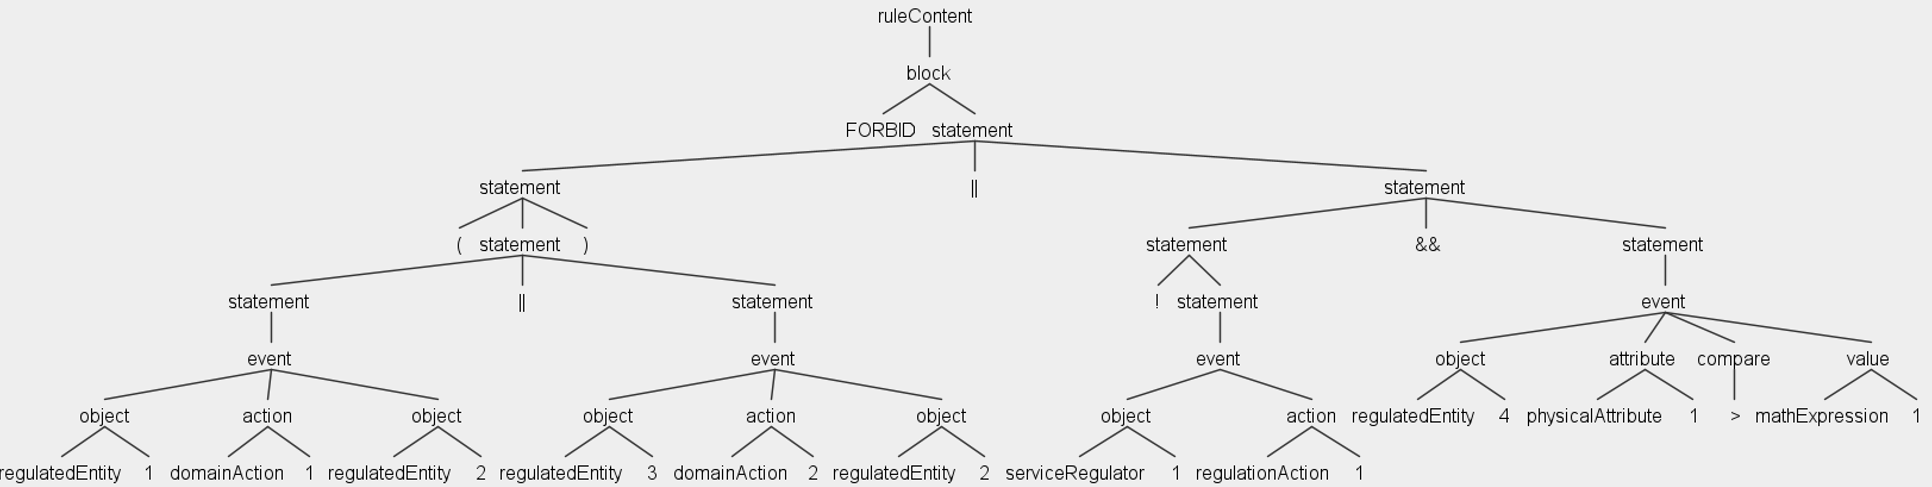
\includegraphics[width=\linewidth]{fig1.png}
\end{figure}

通过Antlr工具,HORAE 的语法分析变得更加系统化和自动化,提高了语言处理的效率和准确性。

\subsubsection{基于大语言模型的语法分析器}

随着研究的不断深入,本研究逐渐认识到,在多样化的数据集面前,Antlr 的解析能力存在一定的局限性。Antlr 擅长构建规范性较强的编程语言的语法分析器,而 HORAE 所面临的规则,往往更接近自然语言的复杂性。对于城市管理等语法结构相对简单的数据集,尚能设计出符合 Antlr 规范的语法规则。然而,面对更广泛的领域和更复杂的基础事件内部结构,遵循 Antlr 的严格规范设计语法就尤为困难。

因此,HORAE 决定保留现有的语法设计框架,同时引入LLMs 进行语法解析,从而突破 Antlr 规范的局限。这种方法使得 HORAE 能够利用 LLMs 在自然语言处理方面的强大能力,以更灵活、更具适应性的方式处理各种复杂的规则内容。

通过在大量文本数据上的预训练,大语言模型已经展现出对自然语言的深入理解,特别是在识别和解析非规范性语言结构方面。通过对这些模型进行微调,HORAE 能够显著提升对特定领域规则内容的解析精度,进而有效提高语法分析器的整体性能。

此外,采用大语言模型还为 HORAE 带来了增量式处理的能力。与需要从头重建的传统编程语言语法分析器不同,大语言模型可以使用 LoRA\cite{hu2021lora}(Low-rank adaptation)技术,保留先前的知识,通过额外的数据集对 LLMs 进行微调,以适应新的事件模式,无需对整个基准数据集重新训练。这一特性极大地增强了 HORAE 的灵活性和可维护性。

有关使用大语言模型进行语法分析的实现细节,请参见 \textbf{\ref{自动化语法分析} 自动化语法分析}。

\newpage

\section{HORAE 语义设计}

HORAE 的语义致力于清晰明确地阐释符合 HORAE 语法的规则所表达的含义。这种语义对于理解和推理通常数量庞大的规则集至关重要。它不仅为监管规则的表示、解释和计算提供了基础,还特别提供了检查规则库的一致性的机制,以便在实际应用到监管任务之前发现并解决潜在的冲突。通过这种方式,可以确保规则库在部署时的可靠性和有效性,避免因规则间的矛盾导致的监管失误。

\subsection{语义建模}

语法设计完成后,规则语言的语义变得清晰:基于语法,逻辑上组合基本事件的可满足性概率。进行语法分析生成解析树后,树的层次结构代表着基本事件之间的逻辑关系。这种逻辑关系可以等同于逻辑表达式。这种模式与SSAT(随机可满足性)模型非常吻合;每个基本事件可以被视为SSAT中的一个布尔随机变量。每个基本事件都有自己的可满足性概率,基本事件之间的逻辑关系直接对应于SSAT中的逻辑运算。因此,本研究以量化的SSAT形式构建了规则语言的语义。

例如,考虑规则 $R1=$ “如果乘客没有房间或者房间干净且湿度标准,则...”,经过语法分析,可以将其分解为 $e1=$ “乘客有房间”,$e2=$ “房间干净”,$e3=$ “房间湿度标准”。然后这个规则的SSAT形式的语义表达可朴素的写为 $R1=\neg e1 \vee e2 \wedge e3$,其语义将是 $P1=1-P(e1)+P(e2)\times P(e3)$。

每条规则是基本事件的逻辑组合,一旦选取部分规则构建了规则子库,它就成为一组命题公式。每个基本事件可以被视为一个命题变量(布尔变量),所有基本事件的集合表示为 $\{e_1, \dots, e_k\}$。因此,规则子库是包含这些基本事件的规则的集合,表示为 $\{r_1, \dots, r_n\}$。设公式为
\begin{align*}
\varphi = \bigwedge_{i=1}^{n} r_i.
\end{align*}

一旦下游服务监管系统完成所有基本事件的系统检测,本模块就获得了一些基本事件子集 $\{e_{i_1}, \dots, e_{i_m}\} \subset \{e_1, ..., e_k\}$ 的赋值集合,表示为 $v: \{e_{i_1}, \dots, e_{i_m}\} \to \{0,1\}$。考虑公式
\begin{align*}
\exists e_{i_{m+1}} \dots \exists e_{i_{k}} \varphi',
\end{align*}
其中 $\{e_{i_{m+1}},\dots,e_{i_{k}}\}=\{e_1,\dots,e_k\} - \{e_{i_1}, \dots, e_{i_m}\}$,且 $\varphi'$ 是用 $v(e_{i_j})$ 替换公式 $\varphi$ 中出现的变量 $e_{i_j}$ 后的结果。如果给定的公式不可满足,则输入数据违反了规则子库。这是一个典型的SAT问题,其语义是:给定一组输入,它们是否满足规则子库中的所有规则。

然而,在现实世界的场景中,服务监管系统的检测模型通常无法准确判断某些基本事件是否满足;它们只能提供事件为真的相应概率。在这种情况下,对于每个命题变量,都有一个相关的概率值,表示其为真的可能性。这种赋值称为“随机赋值”。给定服务监管系统一组输入数据(可能是多模态的:文本、图像或视频),可以对所有基本事件 $\{e_{i_1}, \dots, e_{i_m}\} \subset \{e_1, ..., e_k\}$ 获得一组随机赋值。设 $p_{i_j}$ 表示基本事件 $e_{i_j}$ 为真的概率。然后,公式
\begin{align*}
    \rotatebox[origin=c]{180}{R}^{p_{i_1}} e_{i_1} \dots \rotatebox[origin=c]{180}{R}^{p_{i_1}} e_{i_m}
    \exists e_{i_{m+1}} \dots \exists e_{i_k}
    \varphi
\end{align*}
具有以下语义:给定输入数据,满足规则子库的最大概率。与确定性逻辑公式相比,这种描述更适合现实生活场景,因为多模态的输入与检测的输出无法完全准确。编码后,这类问题的模式与SSAT(随机布尔可满足性)问题一致。因此,本研究使用SSAT求解器来解决这个问题。

\subsection{相似性检验}

在根据 HORAE 解析规则时,基本事件相关性仍然是一个挑战:来自同一规则库 的基本事件在自然语言方面可能彼此语义相关或相同,尤其是跨不同规则语句的基本事件。那么如何将这些用自然语言描述的事件抽象成一组符号命题,同时保证语义相关性呢?实际上,这可以通过在自然语言处理中用于评估文本相似性的多种技术来实现,例如 TF-IDF\cite{ramos2003using}、Word2Vec\cite{sivakumar2020review},以及 BERT\cite{koroteev2021bert}。在一系列的测试中,SBERT 的性能表现最佳。

\begin{figure*}[ht]
\begin{align*}
    s_1 &= \underbrace{\text{员工请求年假}}_{\textcolor[rgb]{0.3, 0.5, 1.0}{e_{11}}} \quad \land \bigg( \underbrace{\text{处于允许期间}}_{\textcolor[rgb]{0.3, 0.5, 1.0}{e_{12}}} \lor \underbrace{\text{经理批准请求}}_{\textcolor[rgb]{0.3, 0.5, 1.0}{e_{13}}} \bigg) \longrightarrow \underbrace{\text{准予假期}}_{\textcolor[rgb]{0.3, 0.5, 1.0}{e_{14}}} \\
    s_2 &= \underbrace{\text{剩余足够假期余额}}_{\textcolor[rgb]{0.3, 0.5, 1.0}{e_{21}}} \land \underbrace{\text{员工提交假期申请}}_{\textcolor[rgb]{0.3, 0.5, 1.0}{e_{22}}} \land \underbrace{\text{经理拒绝申请}}_{\textcolor[rgb]{0.3, 0.5, 1.0}{e_{23}}} \longrightarrow \underbrace{\text{需要行政复核}}_{\textcolor[rgb]{0.3, 0.5, 1.0}{e_{24}}} \\
    s_3 &= \bigg( \underbrace{\text{假期余额耗尽}}_{\textcolor[rgb]{0.3, 0.5, 1.0}{e_{31}}} \lor \underbrace{\text{员工申请年假权利}}_{\textcolor[rgb]{0.3, 0.5, 1.0}{e_{32}}} \bigg) \land \underbrace{\text{申请在限制期间内}}_{\textcolor[rgb]{0.3, 0.5, 1.0}{e_{33}}} \longrightarrow \underbrace{\text{请求自动拒绝}}_{\textcolor[rgb]{0.3, 0.5, 1.0}{e_{34}}}
\end{align*}
\caption{相似性检验的样例,对于以上三条规则,各包含四个基础事件,其中有表述不同但本质一致的情况:${\textcolor[rgb]{0.3, 0.5, 1.0}{e_{11}}} = {\textcolor[rgb]{0.3, 0.5, 1.0}{e_{22}}} = {\textcolor[rgb]{0.3, 0.5, 1.0}{e_{32}}}$, ${\textcolor[rgb]{0.3, 0.5, 1.0}{e_{12}}} = \neg {\textcolor[rgb]{0.3, 0.5, 1.0}{e_{33}}}$, ${\textcolor[rgb]{0.3, 0.5, 1.0}{e_{13}}} = \neg {\textcolor[rgb]{0.3, 0.5, 1.0}{e_{23}}}$, ${\textcolor[rgb]{0.3, 0.5, 1.0}{e_{21}}} = \neg {\textcolor[rgb]{0.3, 0.5, 1.0}{e_{31}}}$, ${\textcolor[rgb]{0.3, 0.5, 1.0}{e_{14}}} = \neg {\textcolor[rgb]{0.3, 0.5, 1.0}{e_{34}}}$,所以需要相似性检验。}
\end{figure*}

以下是利用SBERT 进行相似性检验的步骤:
\begin{itemize}
    \item \textbf{数据预处理:} 将规则库中的所有基本事件提取出来,并进行必要的文本清洗,包括去除停用词、标点符号,以及执行词干提取或词形还原。
    \item \textbf{向量化表示:} 使用 SBERT 将每个清洗后的基本事件转换为固定长度的向量表示。这些向量能够捕捉事件之间的语义相似性。
    \item \textbf{相似性度量:} 计算每一对基本事件向量之间的相似度。这可以通过余弦相似度、欧氏距离或其他相似性度量方法来实现。
    \item \textbf{相似性阈值设定:} 为了确定两个事件是否足够相似,需要设定一个相似性阈值。如果两个事件的相似度超过这个阈值,则认为它们是一致的。需要注意的是阈值的设置需要非常保守,服务监管系统能够接受的本质一致的基本事件被认为不同,这只会导致性能的下降;但本质不同的基础事件被认为是一致的将会导致错误的出现。
\end{itemize}

通过这种方法,本研究能够有效地处理来自同一规则库的基本事件之间的语义相关性,从而提高规则库的一致性和可管理性。此外,SBERT 的使用还为本研究提供了一种灵活的方式来适应不同的规则库和领域,因为它们可以被训练或微调以适应特定的语料库或领域术语。

SBERT 的性能会受到训练数据质量和模型参数的影响。因此,实际应用需进行充分的测试和调整,以确保获得最佳的相似性检验结果。

\subsection{一致性检验}

一致性验证的目的是确定给定的规则库是否包含相互冲突的多个规则。当规则库中的所有规则都能同时被满足时,该规则库就是一致的。验证规则库一致性的核心思想是将其转化为一个布尔可满足性问题(SAT)。首先,将基本事件视为布尔变量,表示为 $e_1, e_2, \ldots, e_k$。然后,可以将由基本事件组成的规则转换为布尔表达式,表示为 $r_1, r_2, \ldots, r_n$。对于给定的规则库,其所有规则可以形成如下的合取范式(CNF):
$$CNF=\bigwedge_{i=1}^{n}r_i=r_1 \land r_2 \land \cdots \land r_n$$

\begin{figure}[!t]
    \centering
    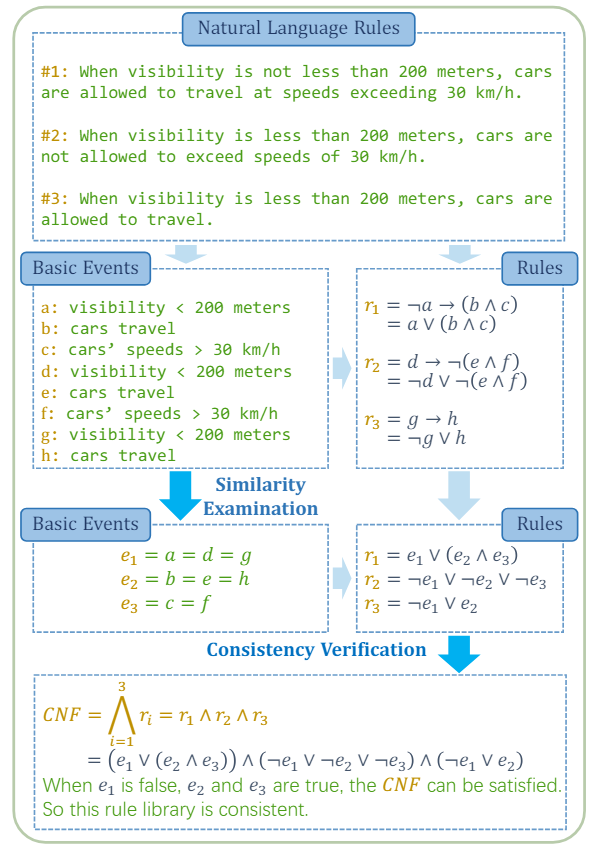
\includegraphics[width=0.7\linewidth]{fig2.png}
    \caption{规则库相似性检验和一致性验证的示例。首先从自然语言规则中解析出所有基本事件,并将这些规则转换为基本事件和逻辑运算符的组合。在完成相似性检验后,所有语义相似(在此示例中为相同)的基本事件被识别并统一为一个符号,该符号可以被视为布尔变量。最后,通过SAT求解器对规则的合取范式(CNF)进行一致性验证。如果存在一组赋值使得布尔变量满足CNF,则规则库是一致的。}
    \label{fig_1}
\end{figure}

Z3求解器可以用来证明这个 CNF 是否可满足,从而验证规则库是否一致。为了进一步说明一致性检验的过程,本研究将其分解为以下几个步骤:

\begin{itemize}
    \item \textbf{布尔变量的赋值:} 为规则库中的每个基本事件分配一个布尔变量,这些变量的真值表示事件是否发生。
    \item \textbf{布尔表达式的构建:} 利用布尔逻辑连接词(如与 $\land$、或 $\lor$、非 $\neg$)将基本事件的布尔变量组合成布尔表达式,以反映规则之间的逻辑关系。
    \item \textbf{合取范式的转换:} 将所有布尔表达式整合成一个合取范式(CNF),这是一个由多个子句构成的逻辑表达式,每个子句由一些变量的析取(或)组成。
    \item \textbf{可满足性求解:} 使用SAT求解器(如Z3)对CNF进行求解,以确定是否存在一组变量赋值,使得整个CNF为真。
    \item \textbf{结果分析:} 如果SAT求解器找到了一个解,则说明规则库是一致的;如果没有找到解,则表明规则库中存在冲突,需要进一步分析和调整。
\end{itemize}

在实际应用中,一致性检验不仅可以帮助服务监管系统确保规则库的逻辑一致性,还可以作为优化和改进规则库的依据。例如,如果发现某些规则之间存在冲突,服务监管系统可以通过修改或重新定义这些规则来解决冲突,从而提高规则库的整体质量和有效性。

总之,一致性检验是确保规则库可靠性和有效性的重要工具。通过将其转化为SAT问题并利用现代求解器的强大能力,可以有效地检测和解决规则库中的潜在冲突,为构建复杂系统和服务提供坚实的基础。

\newpage

\section{自动化语法分析}\label{自动化语法分析}

将自然语言规则自动化语法分析到 HORAE 规范下是服务监管系统关键的一步。考虑到当前预训练语言模型的流行以及它们对自然语言的理解,本文提出了一种基于微调大语言模型的分步解析方法,下文将其称为 \textbf{ParseGPT}。

\begin{figure*}[ht]
\centering
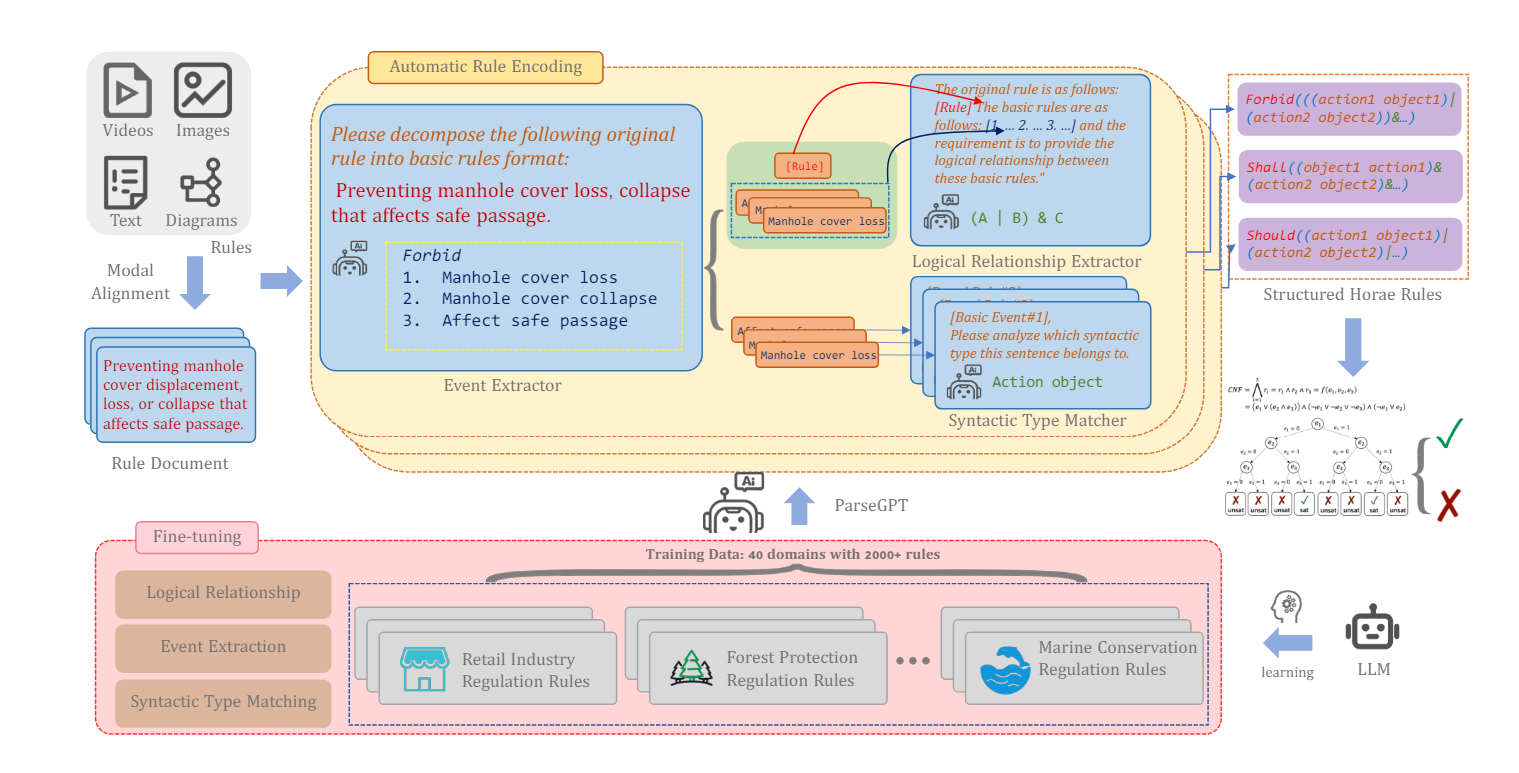
\includegraphics[width=\linewidth]{fig3.png}
\caption{自动化语法分析的全过程}
\end{figure*}
该方法涉及对原始自然语言规则执行三个关键操作:基本事件提取、逻辑关系提取和基本事件模式匹配。实验表明,直接利用大语言模型同时执行这三项操作,即使采用 GPT-4\cite{achiam2023gpt},也无法获得满意的结果。这是因为语法分析过程需要复杂的逻辑推理,在零样本或少样本学习条件下,大语言模型难以迅速掌握语法分析逻辑和方法。为此,本文采取了微调的预训练语言模型\cite{edunov2019pre}(pre-trained language
model,PLM)并采用分段式语法分析策略来解决这一特定问题。具体而言,整个过程被划分为以下三个部分:
\begin{figure*}[ht]
    \centering
    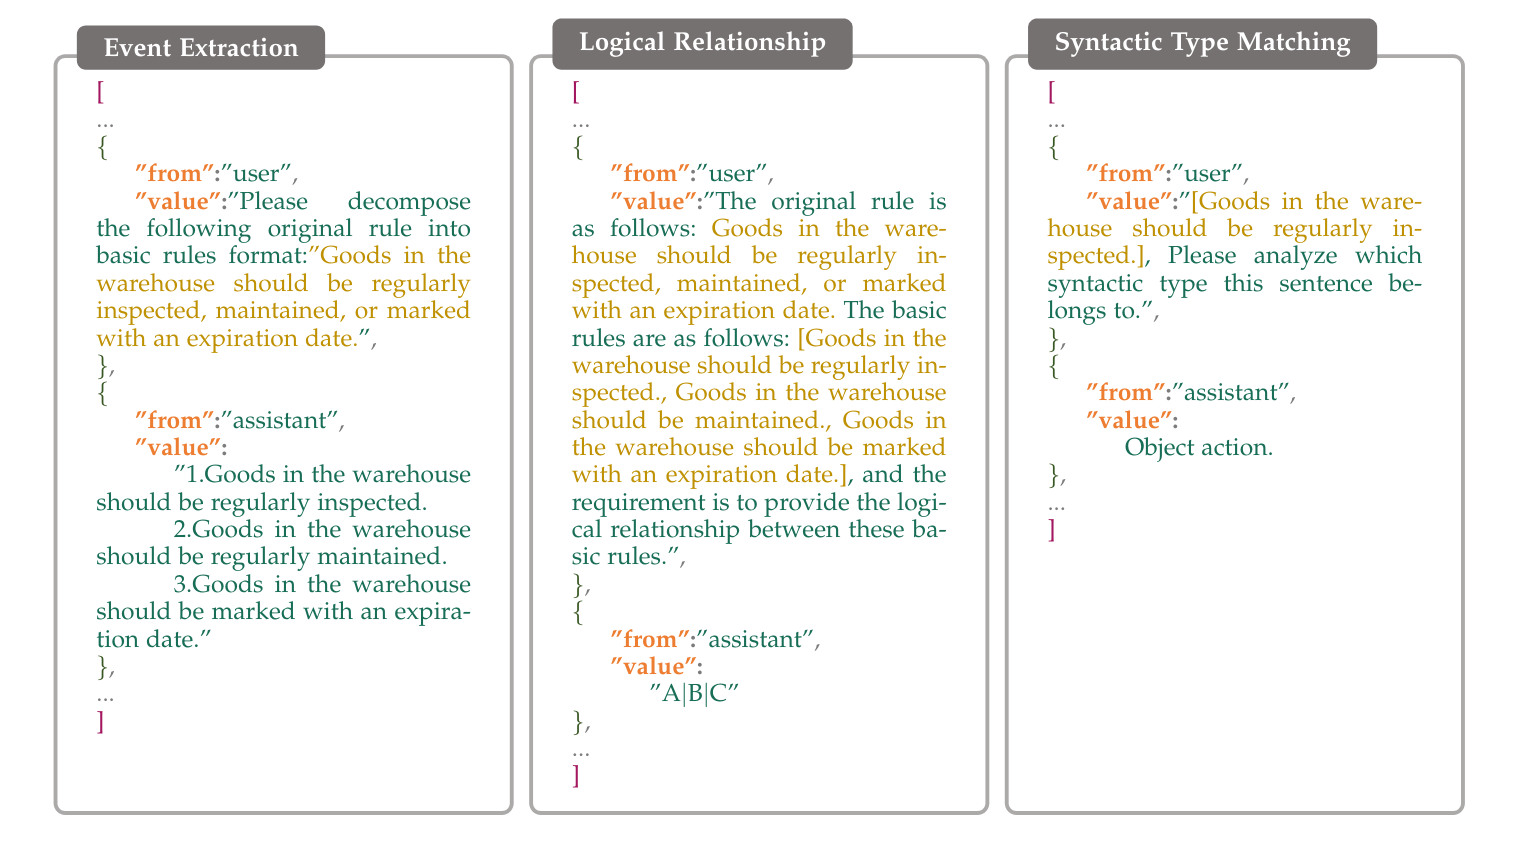
\includegraphics[width=\linewidth]{fig4.png}
    \caption{自动化语法分析的三个部分}
    \label{fig111}
    \end{figure*}
\subsection{基本事件提取}
自动化语法分析的第一步是基本事件提取。尽管基本事件仍以自然语言表达,且同一事件可能存在不同的表达形式,但这并不影响自动化语法分析的后续步骤。在基本事件模式匹配阶段,将本步骤中提取的基本事件与形式化语法相匹配,使得不同的语言表达形式在形式化表示中得以统一。在模型评估阶段,需要一种有效的方法来量化评估训练模型的基本事件提取能力。传统方法通常涉及使用诸如 BERT 的编码器对不同句子进行编码,并在特定向量空间中计算编码后的距离,距离越近表示句子间的相似度越高。然而,在自然语言规则的特定情境中,微小的语言差异可能导致显著的语义差异。为应对这一问题,本研究考虑采用 SBERT 方法来衡量两个基本事件之间的语义相似性。SBERT 是 BERT 的优化版本,在语义相似性任务上的性能得到了显著提升。在特定模型训练中,本项目选择了 Qwen-7B\cite{bai2023qwen} 这一开源预训练模型,并采用 Lora 方法进行微调。微调训练数据采用 JSON 格式,数据来源为FRR-Eval中的第一类数据集。每个训练样本遵循问-答模式;"user" 提出特定提示示例,"assistant" 提供所需的分解形式,如\autoref{fig111}中 Event Extraction。

\subsection{逻辑关系提取}

逻辑关系提取是自动化语法分析的重要组成部分。在基本事件提取完成后,需要正确地通过逻辑关系符号连接基本事件。这不仅影响语法分析的准确性,还影响服务监管系统的下游应用。在实际应用场景中,下游任务将评估每个基本事件的发生概率并返回结果。在获得基本事件的概率后,需要使用正确的逻辑关系符号来计算规则违规(以及合规)的总体概率。因此,正确的逻辑关系在很大程度上决定了语法分析结果的质量。本步骤继续使用相同的预训练模型和相同的 Lora 方法进行微调。微调训练数据也以 JSON 文件中的问-答模式呈现,如\autoref{fig111}中 Logical Relationship。值得注意的是,在逻辑关系提取和基本事件提取的训练中,都使用了 FRR-Eval 中的第一类数据集。原因在于这两个任务具有相同的核心:模型只有在真正理解逻辑关系后才能正确提取基本事件,二者是相互依存的。在构造 FRR-Eval 数据集时,第一类数据集中的基本事件本身在语法上非常简单,适用于分解能力和逻辑理解的训练。

\subsection{基本事件模式匹配}

基本事件模式匹配作为自动化语法分析过程的最后一步,标志着从自然语言规则到规范化格式的最终过渡。由于 HORAE 中定义的基本事件模式数量有限,因此这项任务本质上可以归纳为一个经典的语句分类问题。在本研究中,本步骤继续使用微调预训练大型模型的方法来实现这一功能。模型和微调方法与之前相同。对于训练数据,本步骤使用 FRR-Eval 中生成的第二类数据集。与第一类不同,第二类数据集是根据基本事件模式创建基本事件的,也旨在避免现实世界中不同基本事件模式的基本事件数量的显著不平衡。微调训练数据如\autoref{fig111}中 Syntactic Type Matching。

\newpage

\section{实验与分析}

本章将通过一系列实验来验证经微调的大语言模型的性能。本研究选用的基线模型为Qwen-7B,对其进行进行微调训练,得到 ParseGPT。实验中将其与原版Qwen-7B、Qwen-14B、GPT-3.5\cite{koubaa2023gpt}进行对比。通过与原版Qwen-7B的对比,可以直观地评估微调过程带来的影响。Qwen-14B则代表了目前开源大语言模型的前沿水平。同时,GPT-3.5则代表了商业大语言模型的前沿进展。本章将进行三组实验,这些实验分别对应于第4章所述自动化语法分析的三个关键步骤。

\subsection{FRR-Eval 数据集}

FRR-Eval 数据集是为了评估和训练大语言模型在自动化语法分析任务中的表现而设计的基准数据集。该数据集包含了来自不同领域的监管规则,用于测试不同模型对 HORAE 的语法分析效果。

数据集收集遵循三个原则:确保不同领域之间的显著异质性,寻找多语言规则数据以评估模型对多种语言的适应性,并确保收集到的规则内容是免费、公开的,可供下载和编辑。

\begin{figure*}[ht]
    \centering
    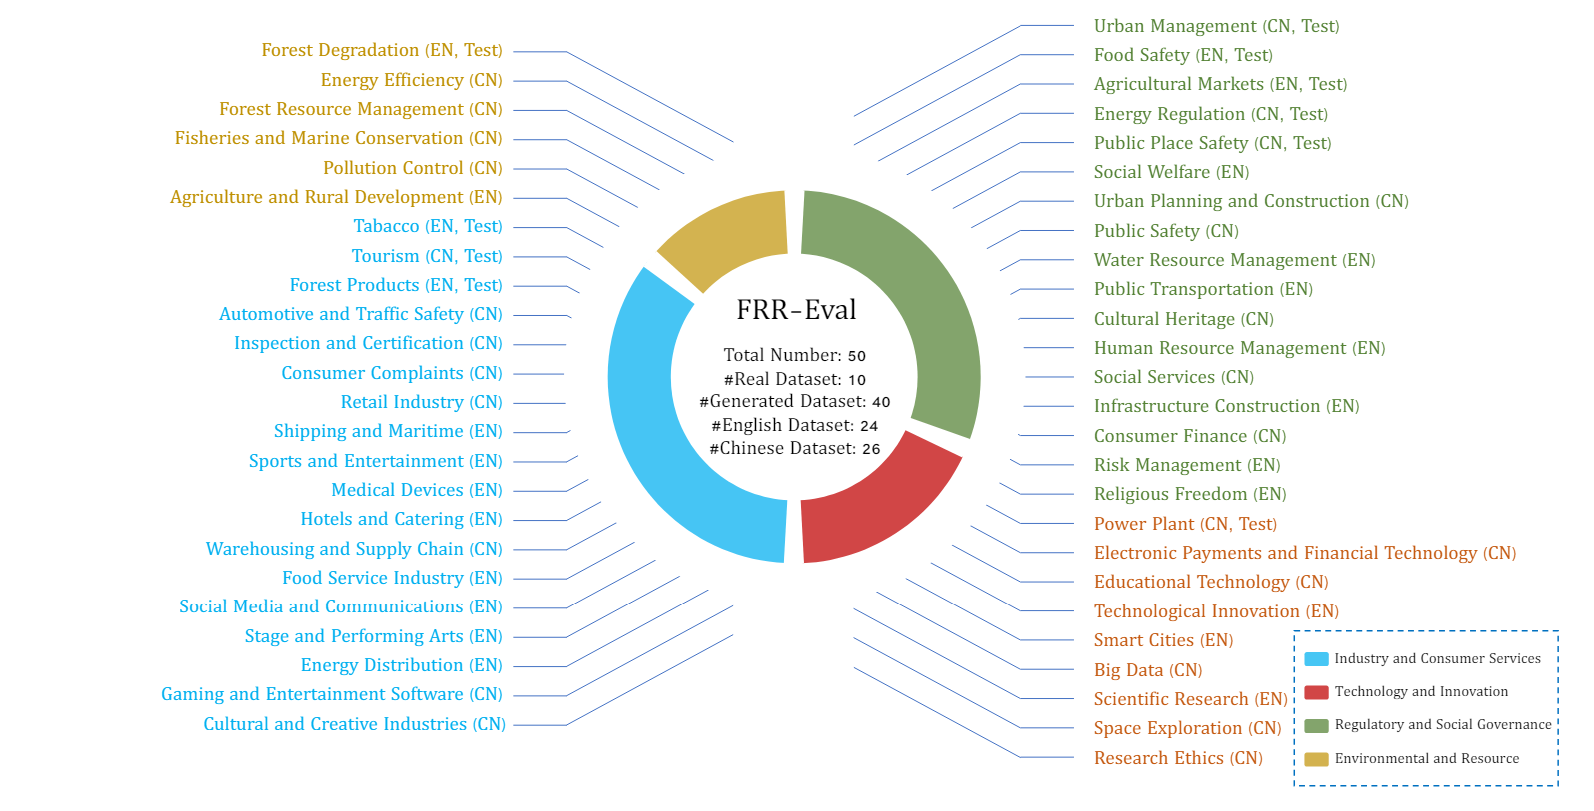
\includegraphics[width=\linewidth]{fig5.png}
    \caption{FRR-Eval 数据集}
\end{figure*}

FRR-Eval 包括了十个真实数据集,涵盖中英文双语境,来源包括城市管理法规、公共法律文件、企业公开文件以及欧盟法律(Eur-lex)。此外,考虑到版权和法律原因,部分领域无法直接公开数据,本研究还使用 GPT-4 结合人工监督生成了四十个常见领域的伪监管规则。

FRR-Eval 数据集包含两种类型的数据:第一种包括规则的原始文本、从这些规则中提取的基本事件列表及其逻辑关系;第二种包括每个领域中各种基本事件及其对应的基本事件模式。这些数据集的作用是训练模型分解原始规则、提取逻辑关系以及将基本事件分类到给定的基本事件模式中。

FRR-Eval 数据集以 JSON 形式全面包含了来自50个领域的监管规则数据,每个领域包含 50 条规则。每个 JSON 对象包含验证集、训练集和测试集,其中验证集包括原始规则、基本事件、逻辑关系和基本事件模式;训练集和测试集包括原始规则数据,用于模型的训练和测试。

为确保标注质量,本研究在任务开始前进行了多对多的数据集标注,并采用 Fleiss Kappa\cite{falotico2015fleiss} 统计量来评估多个标注者在对数据进行标注时的可靠性和一致性。在进行质量评估时,选择了森林资源管理和城市管理两个领域,其 Fleiss Kappa 值分别为 0.845 和 0.864,说明数据标注的可靠性一致性达标。

\subsection{基本事件提取能力测试}

本实验对于四种模型在基本事件提取方面的能力进行了比较。由于无法直接判断事件的拆分是否正确,本研究采用了基于SBERT相似度得分的加权评估指标。这些指标包括加权正确率(wa)、加权召回率(wr)和加权F1分数(wf1),它们综合考虑了事件之间的语义相似性,从而为模型性能提供了全面评估。

加权正确率(wa)的计算公式如下:
\[ P_w = \frac{1}{N} \sum_{i=1}^{N} s(e_i, e'_i) \]

其中,\( N \) 是模型生成的基本事件总数,\( e_i \) 是模型生成的第 \( i \) 个基本事件,\( e'_i \) 是与 \( e_i \) 最相似的原始基本事件。\( s(e_i, e'_i) \) 是它们之间的SBERT相似度得分。若 \( e'_i \) 不存在,则 \( s(e_i, e'_i) = 0 \)。

加权召回率的计算公式如下:
\[ R_w = \frac{1}{M} \sum_{j=1}^{M} s(e'_j, e_j) \]

其中,\( M \) 是数据集中原始基本事件的总数,\( e_j \) 是数据集中的第 \( j \) 个基本事件,\( e'_j \) 是模型生成的与 \( e_j \) 最相似的基本事件。\( s(e'_j, e_j) \) 是它们之间的SBERT相似度得分。若 \( e_j \) 不存在,则 \( s(e'_j, e_j) = 0 \)。

加权F1分数是加权正确率和加权召回率的调和平均值,其计算公式如下:
\[ F1_w = 2 \cdot \frac{P_w \cdot R_w}{P_w + R_w} \]

实验结果如\autoref{tab:111}所示。显然,ParseGPT在正确率(wa)指标上表现尤为出色,在九个数据集中取得了最佳结果。然而,在召回率(wr)指标上,ParseGPT略逊于GPT-3.5和Qwen-14B-Chat模型。在相对全面的'wf1'指标上,ParseGPT始终取得最佳或次佳成绩,显著超越了基线模型Qwen-7B-Chat的性能。值得注意的是,ParseGPT在所有中文数据集中均排名第一,而在英文数据集中则被GPT-3.5超越。这可能归因于ParseGPT的基线模型Qwen-7B-Chat更倾向于中文语料,而GPT-3.5则更倾向于英文语料。

\begin{table*}[ht]
    \centering
    \caption{基本事件提取表现}
    \label{tab:111}
    \resizebox{\textwidth}{!}{
    \begin{tabular}{@{}lcccccccccccc@{}}
    \toprule
     & \multicolumn{3}{c}{Qwen-7B-Chat} & \multicolumn{3}{c}{Qwen-14B-Chat} & \multicolumn{3}{c}{GPT-3.5}  & \multicolumn{3}{c}{ParseGPT} \\
    \cmidrule(lr){2-4}
    \cmidrule(lr){5-7}
    \cmidrule(lr){8-10}
    \cmidrule(l){11-13}
         & wa & wr & wf1 &  wa & wr & wf1 & wa & wr & wf1 & wa & wr & wf1  \\
    \midrule
    发电厂(中文) &0.48  &0.54  &0.51  &0.53  &0.61  &0.57  &0.63  &\textcolor{red}{0.70}  &0.66  &\textcolor{red}{0.79}  &0.60  &\textcolor{red}{0.68}   \\
    公共场所安全(中文) &0.46  &0.61&0.52  &0.60  &0.75  &0.67&0.73  &\textcolor{red}{0.80}  &0.76  &\textcolor{red}{0.86}  &0.73  &\textcolor{red}{0.79}    \\
    旅游(中文) &0.58  &0.61  &0.60  &0.52  &0.67  &0.58  &0.68  &0.55  &0.61  &\textcolor{red}{0.83 } &\textcolor{red}{0.69 } &\textcolor{red}{0.75 }   \\
    能源监管(中文) &0.49  &0.43  &0.46  &0.61  &0.54  &0.57  &0.59  &\textcolor{red}{0.56}  &0.57  &\textcolor{red}{0.81}  &0.48 &\textcolor{red}{0.60  }  \\
    城市管理(中文) &0.50  &0.57  &0.53  &0.56  &0.71 &0.63  &0.74  &\textcolor{red}{0.82}  &0.78 &\textcolor{red}{0.85}  &0.74  &\textcolor{red}{0.79  }  \\
    林产品(英文) &0.32  &0.40  &0.35  &0.33  &0.40  &0.36  &0.54  &\textcolor{red}{0.53}  &\textcolor{red}{0.54}  &\textcolor{red}{0.63}  &0.42  &0.51   \\
    烟草(英文) &0.35  &0.42  &0.38  &0.38  &0.49  &0.43  &0.54  &\textcolor{red}{0.64}  &\textcolor{red}{0.59}  &\textcolor{red}{0.72}  &0.47  &0.57   \\
    农产品市场(英文) &0.32  &0.37  &0.34  &0.36  &0.40  &0.38  &0.53  &\textcolor{red}{0.47}  &\textcolor{red}{0.50}  &\textcolor{red}{0.56}  &0.32  &0.41    \\
    食品安全(英文) &0.25  &0.39  &0.31  &0.33  &0.44  &0.38  &0.47  &\textcolor{red}{0.53}  &\textcolor{red}{0.50}  &\textcolor{red}{0.48}  &0.47  &0.47    \\
    森林退化(英文) &0.34  &0.41  & 0.37 &0.37  &0.40  &0.38  &\textcolor{red}{0.54}  &\textcolor{red}{0.48}  &\textcolor{red}{0.51}  &0.42  &0.36  &0.40  \\
    \bottomrule
    \end{tabular}
    }
\end{table*}

\subsection{逻辑关系提取能力测试}

本实验对于四种模型在逻辑关系提取方面的能力进行了比较。在零样本学习的前提下,手动审查模型输出的逻辑关系,只要模型最终能够提供基本事件之间的正确逻辑关系,不论其表达方式如何,均视为正确。\autoref{tab:222}展示了四种模型在不同数据集上的正确率。

显然,ParseGPT在所有十个数据集上都拥有绝对优势,显著超过了GPT-3.5在提取逻辑关系方面的能力。值得注意的是,ParseGPT的基线模型Qwen-7B-Chat几乎无法识别任何逻辑关系。这反映了微调大语言模型的有效性。

% \begin{table*}[ht]
% \centering
% \caption{逻辑关系提取正确率}
% \label{tab:222}
% \begin{tabular}{@{}lccccccccc@{}}
% \toprule
% & {Qwen-7B-Chat} & {Qwen-14B-Chat} & {GPT-3.5}  & {ParseGPT} \\
% \midrule
% 发电厂(中文) & 0.02 & 0.16 & 0.38  & \textcolor{red}{0.54} \\
% 公共场所安全(中文) & 0.04 & 0.27 & 0.57  & \textcolor{red}{0.86} \\
% 旅游(中文) & 0.02 & 0.18 & 0.40  &\textcolor{red}{0.76} \\
% 能源监管(中文) & 0 & 0.11 & 0.24  & \textcolor{red}{0.56} \\
% 城市管理(中文) & 0.12 & 0.34 & 0.38  & \textcolor{red}{0.58} \\
% 林产品(英文) & 0.02  & 0.26  & 0.34  & \textcolor{red}{0.50}     \\
% 烟草(英文) & 0.02  & 0.28  & 0.36  & \textcolor{red}{0.64}    \\
% 农产品市场(英文) & 0  & 0.28  & 0.34  & \textcolor{red}{0.54}     \\
% 食品安全(英文) & 0.06  & 0.36  & 0.48  & \textcolor{red}{0.52}     \\
% 森林退化(英文) & 0.04  & 0.18  & 0.16  & \textcolor{red}{0.46}   \\
% \bottomrule
% \end{tabular}
% \end{table*}
\begin{longtable}{@{}lccccccccc@{}}
    \caption{逻辑关系提取正确率} \label{tab:222} \\
    \toprule
     & \textbf{Qwen-7B-Chat} & \textbf{Qwen-14B-Chat} & \textbf{GPT-3.5} & \textbf{ParseGPT} \\ 
    \midrule
    \endfirsthead
    
    \toprule
     & \textbf{Qwen-7B-Chat} & \textbf{Qwen-14B-Chat} & \textbf{GPT-3.5} & \textbf{ParseGPT} \\ 
    \midrule
    \endhead
    
    \midrule
    \endfoot
    
    \bottomrule
    \endlastfoot
    
    发电厂(中文) & 0.02 & 0.16 & 0.38 & \textcolor{red}{0.54} \\
    公共场所安全(中文) & 0.04 & 0.27 & 0.57 & \textcolor{red}{0.86} \\
    旅游(中文) & 0.02 & 0.18 & 0.40 & \textcolor{red}{0.76} \\
    能源监管(中文) & 0 & 0.11 & 0.24 & \textcolor{red}{0.56} \\
    城市管理(中文) & 0.12 & 0.34 & 0.38 & \textcolor{red}{0.58} \\
    林产品(英文) & 0.02 & 0.26 & 0.34 & \textcolor{red}{0.50} \\
    烟草(英文) & 0.02 & 0.28 & 0.36 & \textcolor{red}{0.64} \\
    农产品市场(英文) & 0 & 0.28 & 0.34 & \textcolor{red}{0.54} \\
    食品安全(英文) & 0.06 & 0.36 & 0.48 & \textcolor{red}{0.52} \\
    森林退化(英文) & 0.04 & 0.18 & 0.16 & \textcolor{red}{0.46} \\
    
\end{longtable}

\subsection{基本事件模式匹配能力测试}

本实验对于四种模型在基本事件模式匹配方面的能力进行了比较。基本事件模式匹配本质上是一个分类任务。如果模型能正确分类类别,则认为正确。\autoref{tab:333}展示了四种模型在不同数据集上的正确率。

可以看出,ParseGPT在大多数数据集中占据主导地位,全面且显著地超过了GPT-3.5的性能,但是在三个数据集中落后于Qwen-14B-Chat。原因可能是这三个数据集的规则特征存在偏向性。例如在“发电厂”的规则数据集中,几乎所有的基本事件模式都是"object action object"。Qwen-14B-Chat倾向于将任何基础事件都匹配为"object action object"的模式,导致在该数据集中的正确率异常偏高。


% \begin{table*}[!t]
% \centering
% \caption{基本事件模式匹配正确率}
% \label{tab:333}
% \begin{tabular}{@{}lcccccccccc@{}}
% \toprule
% 数据 & {Qwen-7B-Chat} & {Qwen-14B-Chat} & {GPT-3.5}  & {ParseGPT} \\
% \midrule
% 发电厂(中文) &0.68  &\textcolor{red}{0.95}  &0.62   &0.69  \\
% 公共场所安全(中文) &0.47 &0.49  &0.13   &\textcolor{red}{0.57}  \\
% 旅游(中文) &0.07 &0.18  &0.17   &\textcolor{red}{0.46}  \\
% 能源监管(中文) &0.67  &0.74  &0.23   &\textcolor{red}{0.77}  \\
% 城市管理(中文) &0.11  &0.13  &0.17   & \textcolor{red}{0.32} \\
% 林产品(英文) &0.17  &0.09  &0.19   &\textcolor{red}{0.48}  \\
% 烟草(英文) &0.17  &\textcolor{red}{0.39}  &0.17   &0.14  \\
% 农产品市场(英文) &0.29  &0.22  &0.08   &\textcolor{red}{0.37}  \\
% 食品安全(英文) &0.12  &0.35  &0.15   &\textcolor{red}{0.36}  \\
% 森林退化(英文) &0.13  &\textcolor{red}{0.31}  &0.17  &0.22  \\
% \bottomrule
% \end{tabular}
% \end{table*}
\begin{longtable}{@{}lccccccccc@{}}
    \caption{基本事件模式匹配正确率} \label{tab:333} \\
    \toprule
    \textbf{数据} & \textbf{Qwen-7B-Chat} & \textbf{Qwen-14B-Chat} & \textbf{GPT-3.5} & \textbf{ParseGPT} \\ 
    \midrule
    \endfirsthead
    
    \toprule
    \textbf{数据} & \textbf{Qwen-7B-Chat} & \textbf{Qwen-14B-Chat} & \textbf{GPT-3.5} & \textbf{ParseGPT} \\ 
    \midrule
    \endhead
    
    \midrule
    \endfoot
    
    \bottomrule
    \endlastfoot
    
    发电厂(中文) & 0.68 & \textcolor{red}{0.95} & 0.62 & 0.69 \\
    公共场所安全(中文) & 0.47 & 0.49 & 0.13 & \textcolor{red}{0.57} \\
    旅游(中文) & 0.07 & 0.18 & 0.17 & \textcolor{red}{0.46} \\
    能源监管(中文) & 0.67 & 0.74 & 0.23 & \textcolor{red}{0.77} \\
    城市管理(中文) & 0.11 & 0.13 & 0.17 & \textcolor{red}{0.32} \\
    林产品(英文) & 0.17 & 0.09 & 0.19 & \textcolor{red}{0.48} \\
    烟草(英文) & 0.17 & \textcolor{red}{0.39} & 0.17 & 0.14 \\
    农产品市场(英文) & 0.29 & 0.22 & 0.08 & \textcolor{red}{0.37} \\
    食品安全(英文) & 0.12 & 0.35 & 0.15 & \textcolor{red}{0.36} \\
    森林退化(英文) & 0.13 & \textcolor{red}{0.31} & 0.17 & 0.22 \\
    
\end{longtable}

\subsection{结论}

经过一系列的实验验证,得出以下结论:

\begin{itemize}
    \item \textbf{微调的有效性:} ParseGPT模型在所有测试任务中均展现出了显著的性能提升,特别是在基本事件提取任务中,其表现显著优于其他模型。这一结果凸显了微调方法在适应特定任务时的有效性,同时也表明了大语言模型在经过适当调整后,能够更好地理解和处理复杂的语言规则。    
    \item \textbf{跨语言的挑战:} 在中英文数据集上的表现分析显示,ParseGPT在处理中文数据集时表现尤为出色,而在英文数据集上虽然略逊于GPT-3.5,但仍保持了较高水平的性能。这一发现揭示了模型在跨语言应用中的潜力与挑战,同时也强调了对特定语言资源和训练策略的需求,以实现更广泛的语言覆盖和更深入的语言理解。    
    \item \textbf{数据集偏差的影响:} 在某些领域的数据集如“发电厂”中,数据出了明显的偏差,这对模型性能产生了影响。尽管Qwen-14B-Chat在这类数据集上表现出色,但ParseGPT的综合性能和稳健性使其在多样化的数据集上更具优势。这一点提示本研究在未来的数据集构建和模型训练中,需要更加关注数据的多样性和平衡性,以提高模型的泛化能力。    
    \item \textbf{自动化语法分析的实践意义:} 实验结果证明了自动化语法分析的可行性,这对于构建智能化监管系统具有重要的实践意义。通过自动化手段将自然语言规则转换为形式化语言,不仅提高了规则管理的效率,也为监管规则的自动执行和实时监控提供了技术支撑。
\end{itemize}

\newpage

\section{总结与展望}

\subsection{工作总结}

本研究提出了服务监管语言 \textbf{HORAE} ,其核心是通过一种结构化且不受特定领域限制的方法,对服务监管规则进行高效建模。这种设计方法不仅增强了系统的管理效率,而且促进了自动化执行,同时满足了跨领域以及多语言环境下的监管需求。HORAE 通过其语法规则和语义设计,能够将复杂的规则转换成机器可解析和执行的格式,从而为服务监管的自动化和智能化打下了坚实的基础。

此外,本研究还进行了自动化语法分析工具ParseGPT的开发,极大地提升了规则转换的效率和准确性。通过在FRR-Eval基准数据集上进行的一系列广泛实验,HORAE 的适用性和分析能力得到了充分验证,其在服务监管领域的广泛应用潜力也得到了显著展示。这些成果不仅推动了服务监管语言的研究发展,也为构建智能化、自动化的监管系统提供了有力的技术支撑。

\subsection{未来发展展望}

HORAE 需致力于提升其模型的泛化能力,使其能够适应更多样和复杂的应用场景。这意味着 HORAE 需要不断地学习和适应新的数据模式,确保在各种不同的服务监管环境中都能保持高效和准确性。

HORAE 的集成也是关键,使其能更好的嵌入到服务监管系统中。使 HORAE 能够实现对服务流程的实时监控,并在必要时自动触发响应机制,从而提高监管的时效性和响应速度。

HORAE 可以进一步开发持续学习和适应新规则的能力,使其能够不断进化,适应监管环境的变化。这将涉及到先进的机器学习技术,使 HORAE 能够从新的数据和反馈中学习,优化自身的监管策略。

作为研究者,需持续推动模型的创新和完善,这不仅包括对现有模型结构的改进和学习策略的调整,还将积极引入最新的人工智能技术。期望能够显著提升 HORAE 的泛化能力,使其在多变的服务监管场景中展现出更高的适应性和准确性。此外,进一步优化 HORAE 的语义检验功能,并致力于将其更紧密地集成到服务监管系统中,以增强其上下文理解力和规则推理的精确度。

综上所述,HORAE 的未来发展将是一个综合性的进程,通过技术创新和跨领域合作,不断提升其作为服务监管语言的性能和应用范围。通过进一步的努力,HORAE 有望成为服务监管领域的重要技术支柱,为实现智能化、自动化的监管提供强有力的支持。